\chapter{Metodología}

\section{Datos}

\subsection{Obtención y análisis exploratorio de datos}

El dataset obtenido esta inicialmente constituido por 585001 tweets, recolectados entre el 22 de mayo y el 22 de junio del 2022, periodo dentro del cual ocurrieron la primera y la segunda vuelta de las elecciones presidenciales en Colombia , el 29 de mayo y 19 de junio respectivamente. Para la extracción de los datos, se utilizaron 173 hashtags con contenido político que tuvieron lugar durante este periodo. Este dataset fue filtrado para remover aquellos tweets que tuvieran menos de 5 palabras, aquellos que tuvieran una proporción de menciones o hashtags mayor al 20\% del total del texto y aquellos que tuvieran links o que provinieran de usuarios con un numero atípico de posteos. Esto redujo la base a 193348 tweets.  Los hashtags utilizados fueron etiquetados en uno de tres sectores políticos: Izquierda, Derecha y Neutro, dependiendo del contenido asociado a dichos hashtags y su tendencia política. En la tabla \ref{table:hashtags} se muestran los hashtags,así como su etiqueta política y cuantos tweets hubo para cada hashtags. En adelante durante el presente trabajo, cuando se hable de sector político, se estará haciendo referencia a esta clasificación.

Cabe resaltar que la asignación de un sector político en particular a un hashtag, fue llevado a cabo a partir de la tendencia política observada en los tweets, lo que no excluye sin embargo la presencia de tweets cuya tendencia política sea contraria. En la tabla \ref{table:ejemplos_1} se pueden encontrar algunos ejemplos de tweets que muestran la relación del hashtag con la orientación política.  El hashtag \#EstallidoSocialEs por ejemplo, fue catalogado como de derecha por presentar en general tweets como el tweet 1 . Sin embargo, hay tweets que lo utilizan, en donde se aprecia un apoyo al candidato de izquierda como el tweet 2 . Del mismo modo el hashtag \#YaEsSuficiente es utilizado en general como apoyo a la izquierda, como en el tweet 3. Sin embargo, también hay casos en donde se usa como apoyo un candidato de derecha como en el ejemplo 4.

\begin{table}
\caption{Ejemplos de tweets con respecto a orientacion politica}
\label{table:ejemplos_1}
\begin{tabular}{{ | p{2cm} | p{13cm} |}}
\toprule
Numero de Ejemplo & Tweet \\
\midrule
1 & @lcvelez @lafm \#EstallidoSocialEs el arma de terror de Petro para obligar a votar por él. \\
2 & Colombia va por el cambio, a redoblar esfuerzos estos 4 días para derrotar a la corrupción. \#PetroYFranciaSonElCambio \#EstallidoSocialEs \\
3 & \#YaEsSuficiente Que los medios proclives al gbno, traten de darle aire boca a boca a un moribundo electoral, FICO. Ante su estancamiento en las encuestas y la distancia que le ha tomado Petro, pretenden en 1 acto de desesperacion, el insuflarlo de votantes de los cuales carece. \\
4 & \#YaEsSuficiente de mentir sobre @ingrodolfohdez , vayan a bucaramanga, vean lo que hizo y ahí si hablen.. \\
5 & \#LoPeorDeEstasElecciones es la división de la gente de este país esta gente y cosas ya que pasan \\
6 & @Zuletalleras Son 4 años O es la. Derecha va realizar un golpe de estado? No cree a sus comentarios son ofensivos e incendiarios.... \#PetroEsPresidente \\
\bottomrule
\end{tabular}
\end{table}

 

La distribución de los hashtags a través de los sectores políticos se puede evidenciar en el gráfico \ref{figure:tweets_cantidad_hashtags} donde se muestra que el sector neutro tiene mas de un  40\% del total de los hashtags, mientras que la izquierda y la derecha, tienen una cantidad semejante, de aproximadamente un 28\% cada uno.


\begin{figure}[t]
	\centering
	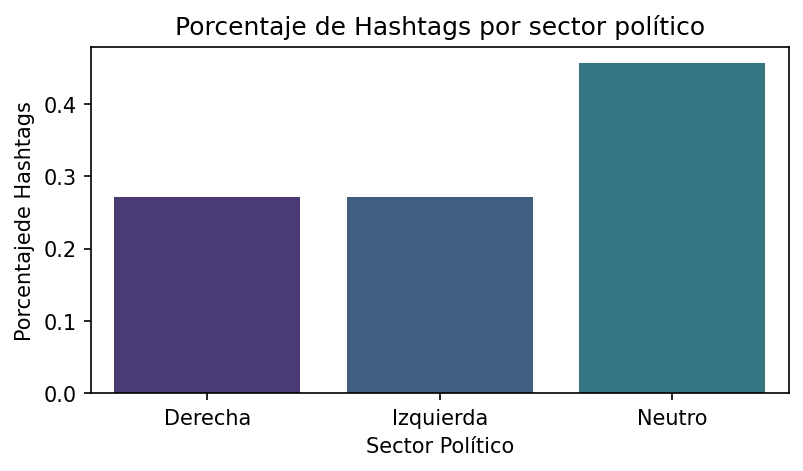
\includegraphics{Images & Logos/EDA/Cantidad de Hashtags por sector politico.png} 
	\caption{Porcentaje de Hashtags clasificados según sector político}
	\label{figure:tweets_cantidad_hashtags}
\end{figure}

De manera similar, el gráfico \ref{figure:tweets_porcentaje} muestra la distribución de tweets a lo largo de los sectores políticos. Allí se aprecia que el sector neutro tiene la mayoría de los tweets, con mas del 46\%, luego se encuentra la izquierda con un 33\% y finalmente la derecha con cerca de un 29\%,



\begin{figure}[t]
	\centering
	\includegraphics{Images & Logos/EDA/Porcentaje de tweets por sector político.png} 
	\caption{Porcentaje de Tweets clasificados según sector político}
	\label{figure:tweets_porcentaje}
\end{figure}


Al analizar la cantidad de tweets por sector político a lo largo del tiempo, se obtienen los resultados observados en el gráfico \ref{figure:tweets_porcentaje_tiempo}, en donde se muestra para cada  sector, que porcentaje del total de los tweets tuvo cada día. Se puede evidenciar que hubo algunas fechas particularmente importantes: el 24 de mayo fue el día de un debate y sobresale el sector neutro, el 29 de mayo fue el día de la primera vuelta y sobresalen los tres, el 9 de junio fue el día en el que salieron a la luz los llamados Petro videos, que fueron unos videos filtrados en donde se ve al equipo de campaña de Petro discutiendo estrategias políticas y sobresale la derecha y las fechas cercanas al 19 de junio que fue la segunda vuelta, sobresalen los tres.




\begin{figure}[t]
	\centering
	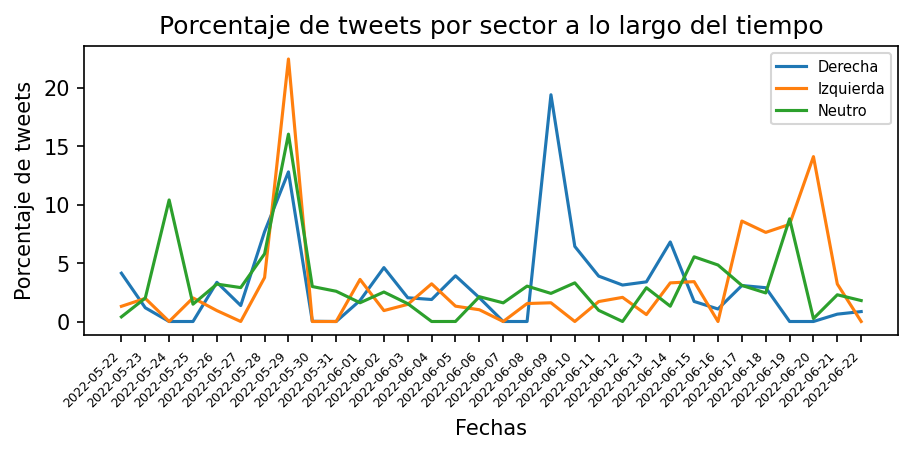
\includegraphics{Images & Logos/EDA/Porcentaje de tweets por sector a lo largo del tiempo.png} 
	\caption{Porcentaje de tweets clasificados según sector político a lo largo del tiempo}
	\label{figure:tweets_porcentaje_tiempo}
\end{figure}



\subsection{Etiquetado}

Para proporcionar un dataset que sirva de base al eventual entrenamiento del modelo , se procedió al etiquetado manual de 1200 tweets escogidos mediante una muestra aleatoria estratificada proporcional a la cantidad de tweets en los hashtags. Las etiquetas a elegir fueron las emociones presentes en el tweet. 

Una emoción es un patrón de reacción complejo, que involucra elementos experienciales, conductuales y fisiológicos, mediante el cual un individuo intenta lidiar con un asunto o evento personalmente significativo. La cualidad específica de la emoción (por ejemplo, miedo, ira) está determinada por el significado específico que el individuo asigna al evento. Por ejemplo, si el evento implica amenaza, es probable que se genere miedo. Están comprendidas de tres componentes distintos: una experiencia subjetiva, una respuesta fisiológica y una respuesta conductual o expresiva.
Para el contexto del presente trabajo, la experiencia subjetiva y la respuesta fisiológica, no son componentes accesibles. Es así como la atención durante el etiquetado recayó en la respuesta expresiva, concretamente, como el autor del tweet, expresa a través del texto, la respuesta emocional generada en respuesta hacia la entidad en particular a la cual se dirige el tweet. 

LA tarea de etiquetado concretamente consistió en etiquetar un tweet a la vez dentro de una plataforma de etiquetado, en donde se tuvo la posibilidad, mediante un esquema de selección múltiple, de asignar una o varias emociones al tweet, basado en los lineamientos presentes en el manual de etiquetado \footnote{\url{https://docs.google.com/document/d/1hoUYKMaYHSeGeOQ2FqRVyahTin6T09Mu8wtl_HY62O0/edit?usp=sharing}}. Esta tarea fue llevado a cabo por el autor y los directores, quedando así 3 etiquetas independiente para cada uno de los tweets.

Para el esquema de etiquetado, se uso como referencia lo elaborado por \cite{mohammad2015sentiment}, en donde el etiquetador responde varias preguntas, y al ser preguntado por la emoción presente en el tweet,  puede escoger 19 emociones distintas. En el presente trabajo a través de una prueba iterativa para elegir las etiquetas mas adecuadas, se llego a escoger 14 emociones posibles ademas de la categoría otra: Alegria, Agrado, Confianza, Admiración, Miedo, Incertidumbre, Sorpresa, Asombro, Tristeza, Decepción, Asco, Desagrado, Ira, Odio, Otra. En la tabla\ref{table:emotions_description} se presenta una descripción de las emociones usadas.

\begin{longtable}{{ | l | p{13cm} |}}
\caption{Descripción de las emociones usadas} \label{table:emotions_description} \\
\toprule
Emoción & Descripción \\
\midrule
\endfirsthead
\caption[]{Descripción de las emociones usadas} \\
\toprule
Emoción & Descripción \\
\midrule
\endhead
\midrule
\multicolumn{2}{r}{Continued on next page} \\
\midrule
\endfoot
\bottomrule
\endlastfoot
Admiración & La admiración es una emoción social que se siente al observar a personas de competencia, talento o habilidad que superan los estándares. La admiración facilita el aprendizaje social en grupos. La admiración motiva la superación personal a través del aprendizaje de los modelos a seguir. \\
Agrado & Sensación moderada de felicidad o placer que siente una persona por algo que le gusta. \\
Confianza & La confianza implica que una parte se vuelve vulnerable ante otra, asumiendo que esta actuará en su beneficio.En una relación de confianza, el que confía no controla las acciones del otro. \\
Alegría & Es una emoción positiva que suele ir acompañada de bienestar. Se genera como resultado de un evento positivo. \\
Incertidumbre & La incertidumbre es la falta de seguridad, de confianza o de certeza sobre algo. Aparece en situaciones en las que no tenemos control total, en las que nos faltan respuestas e información, y nos puede generar inquietud, inseguridad, estrés, ansiedad e incluso miedo \\
Miedo & El miedo surge ante amenazas reales o imaginarias de daño físico, emocional o psicológico. En textos, se muestra como amenazas hacia el autor del mensaje o lo que se menciona, cuando está vulnerable o en desventaja.  \\
Asombro & La condición de estar asombrado; un estado de asombro abrumador, como por sorpresa o miedo repentino, horror o admiración.  \\
Sorpresa & Se define como una reacción provocada por algo inesperado, extraño o novedoso para la persona. En el texto está principalmente asociada a resultados inesperados o descubrimientos singulares respecto al enunciado del tweet. \\
Decepción & La decepción es la insatisfacción que sigue al fracaso de expectativas o esperanzas. A diferencia del arrepentimiento que se centra en elecciones personales, la decepción se enfoca en el resultado en sí. Puede generar estrés psicológico. \\
Tristeza & La tristeza es un dolor emocional causado por decadencia espiritual, manifestándose en llanto, abatimiento, falta de apetito, cansancio, etc. Ocurre cuando las expectativas no se cumplen o las circunstancias son dolorosas.  \\
Desagrado & Una actitud o un sentimiento de disgusto o aversión. \\
Asco & Contiene una serie de estados con intensidades variables que van desde una leve aprensión hasta una intensa repulsión. Todos los estados de asco se desencadenan por la sensación de que algo es aversivo, repulsivo y/o tóxico.  \\
Odio & El odio es una intensa respuesta emocional negativa hacia ciertas personas, cosas o ideas, generalmente relacionadas con la oposición o repulsión hacia algo. El odio a menudo se asocia con intensos sentimientos de ira, desprecio y disgusto. \\
Ira & La ira surge por objetivos no alcanzados o trato injusto, pudiendo ser peligrosa y relacionada con la violencia. En el texto, el autor reta o reclama por un derecho vulnerado, buscando justicia. \\
\end{longtable}



Este etiquetado se llevo a cabo usando la plataforma web Label Studio. La interfaz de etiquetado se puede observar en la figura \ref{figure:interfaz}.


\begin{figure}[t]
	\centering
	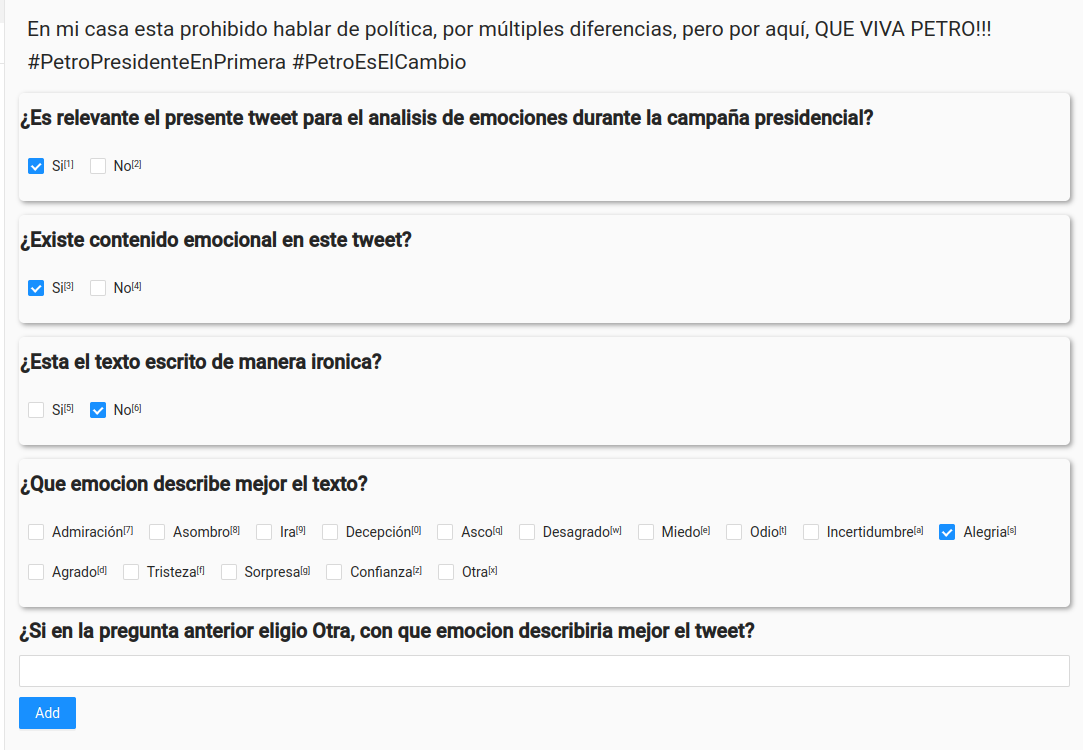
\includegraphics[scale=0.45]{Images & Logos/interfaz.png}
	\caption{Interfaz de etiquetado} 
	\label{figure:interfaz}
\end{figure}

A partir de los resultados obtenidos, se obtuvo el gráfico \ref{figure:correlacion_emociones}, en donde  se calcula la correlacion que tuvieron las etiquetadores en las distintas etiquetas. 

\begin{figure}[t]
	\centering
	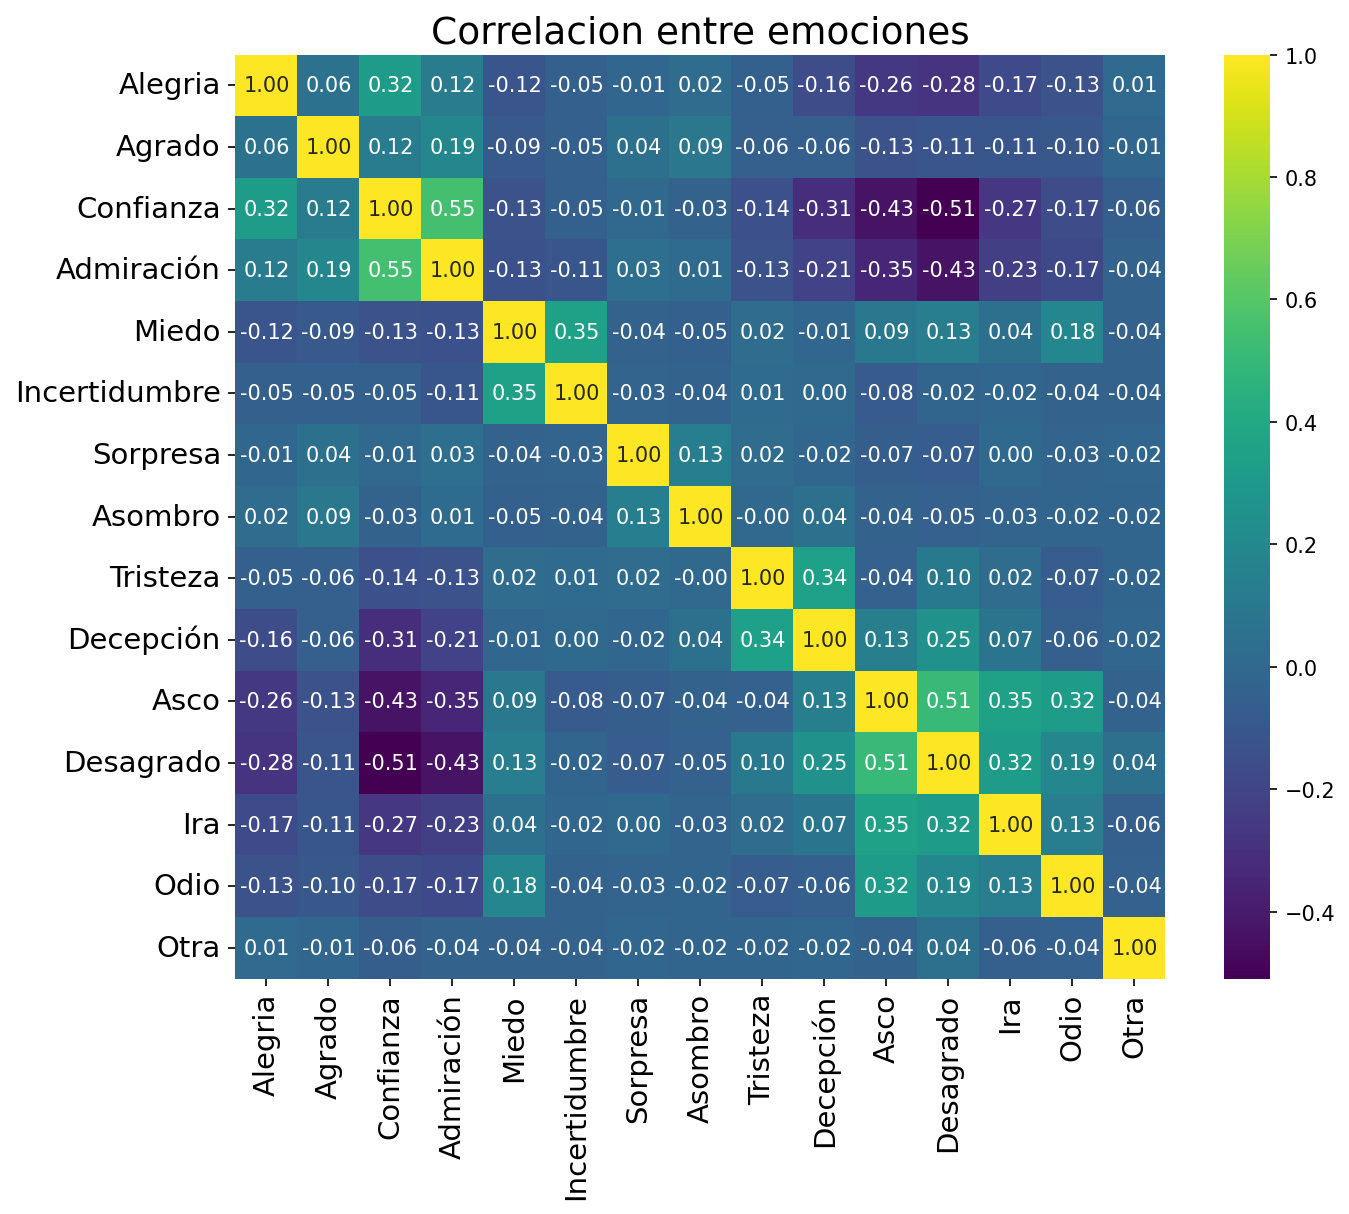
\includegraphics[scale=0.65]{Images & Logos/EDA/emotions_correlations.png} 
	\caption{Porcentaje de coorelación entre etiquetadores de las emociones asignadas a los tweets'}
	\label{figure:correlacion_emociones}
\end{figure}


Basándose en estos resultados, se construyeron 4 etiquetas agrupadoras, a partir de la correlacion que presentaron. Estas etiquetas fueron: Alegría que contiene las etiquetas Alegria, Agrado, Confianza y Admiración; Miedo que contiene las etiquetas Miedo e  Incertidumbre; Tristeza que contiene las etiquetas Tristeza y  Decepción; y 
Asco que contiene las etiquetas Asco, Desagrado, Ira y Odio. A cada tweet se le asigno una o varias de estas etiquetas finales, si al menos dos de los etiquetadores coincidían en dichas etiquetas. Estas fueron las etiquetas con las que se entreno el modelo.

El acuerdo observado entre los etiquetadores para cada una de estas 4 emociones, fue medido utilizando el indice de Fleiss Kappa. Los resultados se encuentran en el cuadro \ref{table:agreements}.


\begin{table}
\caption{Indice de Fleiss Kappa en cada emocion}
\label{table:agreements}
\centering
\begin{tabular}{lllll}
\toprule
 & alegria & miedo & tristeza & asco \\
\midrule
Cantidad de Tweets & 464 & 98 & 103 & 580 \\
Indice de Fleiss Kapp & 0.69 & 0.47 & 0.4 & 0.62 \\
\bottomrule
\end{tabular}
\end{table}


Se puede apreciar como alegría y asco tuvieron puntajes relativamente altos en comparación con tristeza y miedo. Esto se explica en parte por la cercanía que presentan estas dos ultimas a ascos, como se puede apreciar en el tweet numero 5 de la tabla \ref{table:ejemplos_1}. En el, dos de los etiquetadores coincidieron en asignar tristeza mientras el tercero asigno asco. Este mismo fenómeno ocurren con miedo como se aprecia en el tweet numero 6 de la tabla. Allí también fue el caso en donde uno de los etiquetadores asigno asco  mientras los otros dos asignaron miedo.


\section{Modelos}

\subsection{Modelos pre entrenados}

Los modelos de lenguaje pre entrenados se encuentran disponibles para su uso en el sitio Hugging Face \footnote{\url{https://huggingface.co/}}. Desde allí, basándose en la relevancia del modelo para la tarea del presente trabajo, se escogieron 6 modelos diferentes para ser probados y escoger aquel que tuviera el mejor desempeño.




\begin{table}
\caption{Descripción de los modelos usados}
\label{table:model_description}
\begin{tabular}{{ | l | l | p{7cm} |}}
\toprule
Modelo & Localizacion & Descripcion  \\
\midrule
robertuito  & pysentimiento/robertuito-base-uncased & Modelo de lenguaje preentrenado para contenido generado por usuarios en español, entrenado siguiendo las pautas de RoBERTa en 500 millones de tweets. \\
bertin & bertin-project/bertin-roberta-base-spanish & Modelo basados en RoBERTa entrenados desde cero en la parte española de mC4 usando Flax \\
electricidad & mrm8488/electricidad-base-discriminator & Electricidad-base-discriminator es un modelo base tipo Electra entrenado en un gran corpus español (también conocido como corpus de BETO) \\
beto & dccuchile/bert-base-spanish-wwm-cased & BETO es un modelo BERT formado en un gran corpus español. BETO tiene un tamaño similar a un BERT-Base y fue entrenado con la técnica de enmascaramiento de palabras completas. \\
roberta & PlanTL-GOB-ES/roberta-base-bne & El roberta-base-bne se basa en el modelo base de RoBERTa y ha sido preentrenado utilizando un corpus en español de 570 GB de texto limpio  \\
twitter-xlm & cardiffnlp/twitter-xlm-roberta-base & Este es un modelo basado en XLM-roBERTa multilingüe entrenado en ~198 millones de tweets y ajustado para el análisis de sentimientos. \\
\bottomrule
\end{tabular}
\end{table}


Los modelos escogidos fueron robertuito \cite{perez-etal-2022-robertuito}, bertin \cite{BERTIN},  BETO \cite{CaneteCFP2020}, electricidad \cite{mromero2020electricidad-base-discriminator},  roberta \cite{ROBERTA} y twitter-xlm \cite{barbieri2022xlm}. En el cuadro \ref{table:model_description} se encuentra una pequeña descripción de estos así como su localización dentro del hub de Hugging Face.




\subsection{Entrenamiento de los modelos}


Debido a que el fine tuning de estos modelos requiere un poder de computo importante, se decidió utilizar el servicio de Google Colab \footnote{\url{https://colab.research.google.com/}}, en donde se pueden desarrollar notebooks utilizando GPU de manera gratuita. Allí, se utilizo la librería Transformers de Huggingface para poder acceder a los modelos. 

Para poder entrenar los modelos con esta librería, existen dos objetos importantes, el Tokenizer y el trainer. El primero, realiza una transformación de los datos de entrada en vectores tokenizados que puedan ser interpretados por el modelo. EL segundo, recibe como entrada estos datos tokenizados, el modelo a utilizar, los hiperparametros y la métrica a utilizar para evaluar el modelo durante el entrenamiento. Tanto para la definición del tokenizer como la del modelo, se debe especificar la ruta del modelo en particular que se desea implementar.

Los modelos se entrenaron usando los hiperparametros por defecto disponibles en Hugging Face. Estos son principalmente Adamw como algoritmo de optimizacion, con un learning rate de 5e-05, un
decay de 0.0, 3 como el numero de epochs en train y un batch size por nucleo de 8. Estos pueden consultarse en el sitio web \footnote{\url{https://huggingface.co/docs/transformers/v4.30.0/en/main_classes/trainer#transformers.TrainingArguments}}

\subsection{Evaluación de los modelos}

Los modelos fueron entrenados y evaluados utilizando la métrica Micro F1 score definida de la siguiente manera:


\[
{\text{Micro F1}}=\frac{\text{TP} }{\text{TP} + \frac{1}{2}\text{(FP +FN)}}
\]

En donde TP es el numero de verdaderos positivos, FP el numero de falsos positivos y FN el numero de falsos negativos a lo largo de todas las clases. Se eligió esta métrica debido a que el modelo en cuestión permite la clasificación múltiple y con esta métrica se puede evaluar de manera simultanea el desempeño de las distintas clases.

Para entrenar y evaluar los modelos, los datos etiquetados se dividieron en train y test. Se opto por no realizar una tercera partición debido a que no se realiza una hiperoptimizacion de los modelos, sumado al tamaño del dataset etiquetado. Una vez particionados los datos, se procedió a entrenar cada uno de los 6 modelos, 10 veces y a guardar el resultado de su desempeño, con el objetivo de obtener una lectura mas robusta, dada la naturaleza aleatoria de las redes neuronales. El resultado del entrenamiento de cada modelo fue registrado en el sitio Wandb \footnote{\url{https://wandb.ai/}}, cuyo propósito es servir de herramienta de acompañamiento al entrenar modelos.






